\documentclass[12pt]{article}

\usepackage{amsmath}
\usepackage{amssymb}
%\usepackage{amsthm}
\usepackage{graphicx}
%\usepackage{float}

\newcommand{\R}{\mathbb{R}}
\newcommand{\V}{\mathbb{V}}
\newcommand{\prl}{\parallel}
\newcommand{\prp}{\perp}

\title{Planar Physics for Computer Simulation\\with Geometric Algebra}
\author{Spencer T. Parkin}

\begin{document}
\maketitle

The goal of this paper is to develop the math and algorithms necessary to perform basic rigid-body dynamics in the plane
using geometric algebra.  As the reader will see, the equations fall out quite nicely under this alternative
mathematical framework.  As we go along we can make comparisons with traditional methods involving
matrices and the cross product.  Geometric algebra (or GA for short) generalizes the inner product by first
developing the notion of the outer product.  An introduction to GA is first given before diving into the
main material.  Readers already familiar with GA can just skip over that part.

\section{Intro to GA}

A GA is constructed using a vector space $\V$, a set of scalars $\R$, addition, and the outer product.  The scalars can be any field,
such as the complex numbers, but since complex numbers arise naturally as a sub-structure of the GA, it makes sense
to just stick with $\R$.

Given a set of $n$ vectors $\{v_i\}_{i=1}^n$ taken from $\V$, we define
\begin{equation}
V = \bigwedge_{i=1}^n v_i
\end{equation}
to be an $n$-blade if the vectors form a linearly independent set, or zero otherwise.
We call $n$ the grade of the blade, and it follows immediately that the dimension of $\V$
is an upper-bound on the highest grade blade we can make that is non-zero.
Also, we let this be an anti-commutative product; a property we'll take advantage of
later on.  This just means that a swap of any two adjacent vectors in a wedge product
will negate the product.

But how do we imagine a blade?  Well, in the case $n=1$, these are already familiar,
because they're just vectors.  In the case $n=2$, you can think of them as pieces
of area.  Similar to vectors, they need not be rooted in any particular location, and
they have an orientation and magnitude.  Unlike vectors, however, they have a non-unique
factorization.  Often, the ability to choose how we factor a blade can make it easier
to algebraically manipulate them in equations in order to work them out.  In the case $n=3$,
you can think of these as pieces of volume, also factorable in many ways, and so on.

Now enters the inner product, and we can understand this product in terms of the
outer product in the sense that it simply does the opposite thing that the outer product
does.  That is, while the outer product builds blades up, the inner product breaks them
down.  You're probably already familiar with the inner product between two vectors (or $1$-blades)
as a scalar value (or $0$-blade), and you already know the geometric interpretation of
this operation.  We are now going to generalize this with higher-grade blades.

First, imagine the outer product as something that extrudes a point ($0$-blade) through
space to make a vector ($1$-blade).  Now use the outer product again to extrude a vector
($1$-blade) through space to make a $2$-blade, and think of it in the shape of a parallelagram.
This parallelagram, though, is not the only one representative of the $2$-blade, remember,
because the factorization in terms of the outer product is not unique.  (Just bare that in mind for now.)
Now extruding the $2$-blade (or parallelagram) again, to get a $3$-blade, or peice of volume,
and think of it in the shape parallelepiped, or even just a box.

Okay, now let's break it down using the inner product.  With each extrusion, a vector was
taken in the outer product with what we had to build it into a higher-grade blade.  We'll now
take what we have in the inner product with a vector to break it down into a lower-grade blade.
As we do this, only the component of the vector parallel to (or in the space of) the blade
will contribute to the operation, while the component of the vector perpendicular to the blade
will play no part.  That is, a vector taken in the inner product with a blade is zero if that vector
is perpendicular to the blade.  If we're working in 3 dimensions, then a vector will always collapse
a $3$-blade into a $2$-blade perpendicular to that vector.  Similarly, another vector can then
collapse the $2$-blade into a vector orthogonal to it, provided it wasn't orthogonal to the $2$-blade.

This has all been a bit hand-wavey so far, so let's be more concrete about it with some algebra.
Given a $2$-blade $B$, and a $1$-blade $v$, let's consider the inner product $v\cdot B$.
We begin by writing
\begin{equation}
v\cdot B = (v_{\prp} + v_{\prl})\cdot B = v_{\prp}\cdot B + v_{\prl}\cdot B = v_{\prl}\cdot B.
\end{equation}
This equation illustrates the fact that only the component $v_{\prl}$ of $v$ parallel to $B$ will
contribute to the operation, since $v_{\prp}\cdot B=0$.  Now, since factorizations of blades
are not unique, we can write $B=v_{\prl}\wedge b$ for some appropriate vector $b$ such
that $v_{\prl}\cdot b=0$.
This is because $v_{\prl}$ is in the space of the blade, which is also to say that $v_{\prl}\wedge B=0$.
We can then define
\begin{equation}
v_{\prl}\cdot B = v_{\prl}\cdot(v_{\prl}\wedge b)\equiv |v_{\prl}|^2 b.
\end{equation}
And there we have it!  How should we interpret this?  Well, I like to think of it as a collapsing
of $B$ into the space of $b$ along the $v_{\prl}$ dimension; the opposite of an extrusion, but it shouldn't be
confused with a projection.  It's not quite that.  We can actually calculate the projection $p$
of $v$ onto $B$ as
\begin{equation}
p = B\cdot v\cdot B^{-1}.
\end{equation}
Note that the inner product is not necessarily associatve in all cases.  Also, what are
we to make of $B^{-1}$?  Neither the inner nor the outer product supports a multiplicative
inverse.  Well, that's where the geometric product comes in.  Given a vector $a\in\V$, and blade $B$,
we define
\begin{equation}
aB \equiv a\cdot B + a\wedge B
\end{equation}
to be the geometric product of $a$ and $B$.  To show that this is invertible, realize that the
product is associative and commutative, and then write
\begin{align}
aaB &= a(a\cdot B) + a(a\wedge B) \\
 &= a\cdot (a\cdot B) + a\wedge (a\cdot B) + a\cdot(a\wedge B) + a\wedge(a\wedge B).
\end{align}
We can now apply some logic.  Clearly, $a\wedge a\wedge B=0$, because a vector repeated
in a list never gives a linearly independent set of vectors.  Also, we must have $a\cdot (a\cdot B)=0$,
because $a$ will be orthogonal to the collapse $a\cdot B$ of $B$ by $a$.  This leaves us
\begin{equation}
aaB = a\wedge(a\cdot B) + a\cdot(a\wedge B).
\end{equation}
Again, applying what we know about the inner and outer products, we see here that in one case,
$B$ is collapsed by $a$, then extruded by $a$; and in another case, $B$ is extruded by $a$, then
collpased by $a$.  In either case, the net result is just some scalar multiple of $B$.  What scalar multiple?
Well, we can also write
\begin{equation}
aaB = (a\cdot a + a\wedge a)B = |a|^2 B.
\end{equation}
To verify this further, we can also write
\begin{align}
aaB &= a\wedge(a\cdot B) + a\cdot(a\wedge B) \\
 &= a_{\prl}\wedge(a_{\prl}\cdot B) + a_{\prp}\cdot(a_{\prp}\wedge B) \\
 &= |a_{\prl}|^2 B + |a_{\prp}|^2 B \\
 &= (|a_{\prl}|^2 + |a_{\prp}|^2)B \\
 &= |a|^2 B.
\end{align}

All in all, we've shown that $a^{-1}=a/|a|^2$, but what about $B^{-1}$ more generally?
Letting $B$ now be an $n$-blade,
a trick for determining $B^{-1}$ is to write $B$ in terms of an orthogonal set of basis vectors $\{b_i\}_{i=1}^n$.
(We then have, for any two distinct integers $i,j\in[1,n]$, the property $b_i\cdot b_j=0$.)
Doing so, we have
\begin{equation}
B = \bigwedge_{i=1}^n b_i = \prod_{i=1}^n b_i.
\end{equation}
Recalling that the outer product is anti-commutative, we also have
\begin{equation}
B = \bigwedge_{i=1}^n b_i = (-1)^k\bigwedge_{i=1}^n b_{n-i+1} = (-1)^k\prod_{i=1}^n b_{n-i+1},
\end{equation}
where $k=n(n-1)/2$ is a triangle number.  Thus,
\begin{equation}
B^2 = (-1)^k\left(\prod_{i=1}^n b_{n-i+1}\right)\left(\prod_{i=1}^n b_i\right) = \prod_{i=1}^n |b_i|^2.
\end{equation}
Finally, we see that
\begin{equation}
B^{-1}=\frac{(-1)^kB}{\prod_{i=1}^n |b_i|^2} = (-1)^k\frac{B}{|B|^2}.
\end{equation}

So far we've covered blades, the inner and outer products, and the geometric product.  The last thing
to cover to give one a general overview of GA is simply a linear combination of blades, which is what
we call a multivector.  Realize that while all vectors are closed under addition, this is not true of blades
in general.  That is, the sum of two blades is not necessarily a blade, even if they have the same grade.
If they do have the same grade, then the result is what we call a $k$-vector.  Every $k$-blade is a
$k$-vector, but not every $k$-vector is a $k$-blade.  In the case $k=1$, we call them vectors; $k=2$,
bivectors; $k=3$ trivectors, and so on.  It's not hard to see why some $k$-vectors are not $k$-blades.
Just add two $2$-blades from partially disjoint vector spaces.

There are many applications of GA; most notably are those of projective and conformal geometry.
In each of these, a vector space of dimension greater than 3 is used to generate a geometric
algebra, and then the projections into 3-dimensional space of the elements of that algebra are studied.
Operations in the higher-dimensional algebra produce geometrically meaningful results in terms of their
"shadows" in 3-dimensional space.  Some are quite fascinating.  For example, in conformal geometric
algebra,\footnote{CGA is patented, by the way, which I think is silly, but whatever.} the outer
product of 4 vectors, each representative of a point in 3-dimensional space, gives an element (a $4$-blade)
representative of the 3-dimensional sphere fitting those 4 points, if the blade is non-zero, of course.
Pretty cool stuff!  Can you think of calculating the sphere fitting 4 given points without such an algebra?

But I believe I've digressed too far.  Let's get back to physics in the plane as
our chosen application of GA.

\section{Rigid Body Model}

For the remainder of the paper, we're going to use $\V=\mbox{span}\{e_1,e_2\}$ as our vector space, where $e_1$ and
$e_2$ denote the $x$ and $y$-axes of the traditional, right-handed cartesian coordinate plane, respectively.  The basis for our GA will
then be
\begin{equation}
\{1,e_1,e_2,e_1\wedge e_2\}.
\end{equation}
That is, the elements of our GA will all be linear combinations of these basis elements.

\subsection{Center of Mass}

For our purposes, a rigid body will be a convex polygon of uniform density.  Convex, because it simplifies collision detection;
and of uniform density, so that mass is a scalar multiple of area.  To make things even simpler, we'll just let mass and area
be the same.

That said, such a rigid body is typically stored in memory as an array of $n$ points $\{x_i\}_{i=1}^n\subset\V$, wound counter-clock-wise in the plane.
Our first order of business will be to calculate its center of mass.  We have to be careful here, because it is tempting to think that $C$ is the center
of mass, where
\begin{equation}\label{equ_geo_center}
C = \frac{1}{n}\sum_{i=1}^n x_i,
\end{equation}
but this is not always the case.  We will let $C$, as it is written here in equation \eqref{equ_geo_center},
denote the average center of our convex shape.  (Note that since
our shape is convex, $C$ is guarenteed to be inside our shape.)
To find the center of mass, however, let's look at its definition.  Given a shape $S$ with area $A$, the center of
mass is given by
\begin{equation}
C = \frac{1}{A}\int_S x dA,
\end{equation}
where here, $dA$ is a bit of area in $S$ at $x$.  Using this definition, we can prove that the center of mass of a right-triangle
is also its average center.
\begin{figure}\label{fig_right_triangle}
\centering
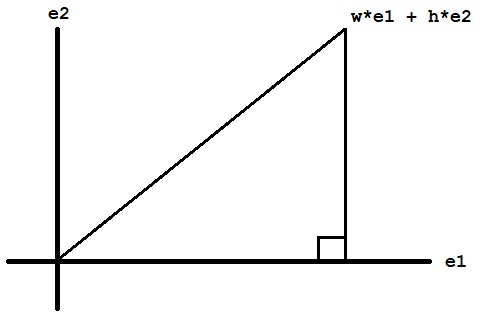
\includegraphics[scale=0.5]{right_triangle}
\caption{A right-triangle in the plane with with $w$ and height $h$.}
\end{figure}
To that end, consider the triangle in figure \eqref{fig_right_triangle}.  The average center of this triangle is clearly
\begin{equation}\label{right_triangle_geo_center}
C = \frac{(0e_1 + 0e_2) + (we_1 + 0e_2) + (we_1 + he_2)}{3} = \frac{2}{3}we_1 + \frac{1}{3}he_2,
\end{equation}
but is this also the center of mass?  To find out, we apply our definition, and come up with the integral
\begin{equation}\label{right_triangle_integral}
C = \left(\frac{wh}{2}\right)^{-1}\int_0^h\int_{yw/h}^w(xe_1 + ye_2)dxdy.
\end{equation}

I'll leave the evaluation of this integral as an exercise for the reader.  Suffice it to say, equations \eqref{right_triangle_geo_center}
and \eqref{right_triangle_integral} should be equal.  Admittedly, I had to scribble this integral on paper a million times before I
finally verified its correctness.  Give it a try if you're skeptical.

With this result in hand, we can now use the following trick to calculate the center of mass of our convex polygon.  First,
we tessellate the convex polygon into a set of $m$ right-triangles $\{T_i\}_{i=1}^m$.  (Tessellate into triangles first, then split each triangle into two right triangles.)
Having done that, let $C(T_i)$ denote the average center of $T_i$, and let $A(T_i)$ denote its area.  The center of mass of our polygon is then
\begin{equation}
C = \frac{1}{A}\sum_{i=1}^m C(T_i)A(T_i),
\end{equation}
where $A=\sum_{i=1}^m A(T_i)$.  This works because each term is the total moments of $T_i$, so the sum is the total moments of our polygon,
and then the center of mass is the total moments of the polygon over its total mass.

Note that another way to compute $A$ is as
\begin{equation}
A = \frac{-e_1e_2}{2}\sum_{i=1}^n (x_i-C)\wedge (x_j-C),
\end{equation}
where $C$ is the average center of the polygon, or really just any interior point of the polygon, and $j=i+1\pmod m$.
A positive result here depends on the counter-clockwise winding of the polygon.

\subsection{Moment of Inertia}

For linear motion we have Newton's famous equation $F=ma$, where $F$ is force, $m$ is mass, and $a$ is acceleration.
Its counter-part in the realm of angular motion is $\tau=I\alpha$, where $\tau$ is torque, $I$ is the moment of inertia, and $\alpha$
is angular acceleration.  Simulating the motion of our rigid body polygon will require us to use these equations.  At this point,
however, we only know the mass of our polygon, and its center of mass (about which it will rotate.)  To know how to rotate
our polygon, we'll also need to know its moment of inertia.

Let's look at the definition.
\begin{equation}
I = \int_S (x-C)^2 dA
\end{equation}
Here, $S$ is our shape in the plane, $dA$ is a bit of area (or mass in our case), $C$ is the center of mass,
and $x$ is our variable of integration, visiting every point of $S$.

It is at this point that I'm at a loss for any kind of trick for calculating the exact value of $I$ for our polygon, and so
what I've done in practice is simply approximate the integral numerically.  This is time-consuming, but it doesn't have
to be done on initialization of your simulation.  It can be done as a build step for the assets loaded by your
simulation.

Note that in 3-dimensions, $I$ is not a scalar, but a tensor matrix, and to make things more complicated, it
depends on the orientation of the rigid body.  We won't have to worry about that in 2-dimensions, though.
Using CGA, the authors of \cite{} found a way to represent the inertial tensor as an element of the algebra.

\subsection{The Equations of Motion}

% Will want the center of mass to be (0, 0) in local space.

Our first goal is to just get our polygons moving realistically through space, with no regard to any external forces or impulses.
After that, we can consider the influence of forces, and resolve collisions using impulses.

% e^{Io/2) w e^{-Io/2} = w e^{Io}, but only in 2D, not in ND.

% Need to add citation for David Baraff here.

\subsection{Resolving Collisions}

\begin{equation}
j = \frac{-(1+\epsilon)(n\cdot (v + r\omega))}{M^{-1}-(r\wedge n)^2/I}
\end{equation}

\begin{equation}
j = \frac{-(1+\epsilon)v_{rel}^{-}}{M_a^{-1}+M_b^{-1}-(r_a\wedge n)^2/I_a - (r_b\wedge n)^2/I_b}
\end{equation}

\end{document}